%!TEX root = ../main.tex

\chapter{Implementation}
\label{chp:implementation}

In this chapter, we will get into the implementation techniques and tricks we employed for the training of our word embedding model. While the theory and design are critical, this is yet another aspect of our work that directly influences the outcome. We will explain the software techniques we used and the reasoning behind our decisions. We will also demonstrate how we implement these ideas in our code. By understanding what we have done to achieve what, the reader will have a better idea about how to reason the strengths and the shortcomings of our model, and what can be done to improve it. We will stick to the notation introduced in the previous chapter when it is needed.

\section{Setup}

We implemented our training and other experiments using Python version 3.10.12, which is one of the most recent versions at the time of this dissertation. Python is a popular choice for projects involving machine learning for reasons such as:
\begin{itemize}
    \item \textbf{Ecosystem}: A wide range of libraries and frameworks that are specifically designed for \ac{NLP} and \ac{ML} tasks. Libraries like \ac{NLTK}, PyTorch, scikit-learn, and TensorFlow provide a wealth of tools for these projects.
    \item \textbf{Ease of Use}: Python is easy to learn and use. Compared to more traditional, lower-level programming languages, it greatly reduces the amount of code required for different tasks. It is known for its elegant and easy-to-read syntax that makes it accessible and easy to collaborate on.
    \item \textbf{Vast Community}: Python has a large and active user community, consisting of professionals from a wide range of domains. One can easily find solutions to even very specific problems and access documentation.
    \item \textbf{Data Manipulation}: There are numerous data manipulation and analysis tools available in Python, which is the backbone of the majority of the \ac{ML} projects. Libraries like NumPy and pandas are common choices for handling and processing large datasets, making it possible to shape the data to the desired format and easily capture interesting properties of the data samples in hand.
\end{itemize}

We practiced cloud computing for this project and used Google Colab as our development environment. Google Colab offers free but limited use of GPU computations. Their free plan grants access to NVIDIA T4 GPU, but for a monthly fee users can also use NVIDIA A100 and V100 paired with a higher memory. Since the computational resources are better and the timeouts are reduced in the paid plan, we subscribed to their paid plan for this study. Google Colab offered several key advantages, including:

\begin{itemize}
    \item \textbf{Portability}: We were able to run our programs from any device connected to the internet, without the need for any installations.
    \item \textbf{Integration with Google Drive}: We stored our files like our logs, datasets, and models on Google Drive, which makes everything more organized and accessible from anywhere in the world.
    \item \textbf{Ease of Collaboration}: Notebooks are quite easy to share, a link can grant access to anyone for viewing or manipulating our experiments, with no downloads or system requirements.
    \item \textbf{Interactivity}: We were able to visualize and modify our code in real-time, which makes it possible to detect and fix errors early on, and rapidly add new ideas to our code.
    \item \textbf{Version Control}: Colab keeps track of the versions of a notebook, making it easier to track changes and go back to an earlier version if needed.
\end{itemize}

We utilized a variety of libraries in our training procedure, but the backbone of our training procedure was built using PyTorch. PyTorch served as the cornerstone of our project, enabling us to define our model architecture and facilitating the crucial process of learning. It not only provided us with a blueprint for our objects but also was crucial for utilizing GPU resources for our multi-dimensional computations. By harnessing the power of PyTorch for machine learning and GPU utilization, NumPy for efficient numerical operations, and Matplotlib for creating visualizations, we successfully crafted, trained, and closely monitored our model's progress and performance.


\section{Preprocessing}
\label{sec:preprocessing}

It is common practice to apply a multi-step preprocessing procedure to the corpus. What we do in this step of our implementation is often called \textit{text normalization}. Text normalization is the process of transforming text-formatted data into a pre-defined form by applying a set of operations in an order. It is crucial to do so for several reasons. For one, just like any other machine learning task, one needs to reformat the data so that the machine learning model can process it. Secondly, a good preprocessing of the training data can greatly enhance the performance of the final product.

Generally, text normalization involves a combination of several tasks. Even though there are general blueprints for specific needs and a catalog of tasks to pick from, the choice greatly depends on the structure of the data and the task at hand. Some of the common tasks include spell checking, contraction, handling punctuation, tokenization, case folding, stop word removal, and stemming. Without going into the details of other possible tasks we could have applied to our data, we will talk about our own procedure.

We are not aiming to produce a case-sensitive model, therefore we start by lower-casing our entire corpus. This way, every occurrence of a type is equalized. This process is also called \textit{case folding}. Even though this is a popular choice for the normalization process, it comes with its downsides. For example, when we lowercase everything, our model will not be able to distinguish some entities such as "cologne", a liquid with a pleasant smell, and "Cologne", a city in Germany. However, we still go for it, considering that it will enable us to utilize our data better in every other case.

\begin{lstlisting}[language=Python, caption=Case folding]
text = text.lower()
\end{lstlisting}

Next, we handle punctuation. We handled punctuation symbols rather than removing them because our belief was that punctuation influences the meanings of linguistic expressions greatly, therefore they are important for lexical meanings as well, especially for a third-order model like ours. By handling punctuation, we mean replacing their occurrences with identifiers.

\begin{lstlisting}[language=Python, caption=Handling Punctuation]
text = text.replace('.', ' <PERIOD> ')
text = text.replace(',', ' <COMMA> ')
text = text.replace('"', ' <QUOTATION_MARK> ')
text = text.replace(';', ' <SEMICOLON> ')
text = text.replace('!', ' <EXCLAMATION_MARK> ')
text = text.replace('?', ' <QUESTION_MARK> ')
text = text.replace('(', ' <LEFT_PAREN> ')
text = text.replace(')', ' <RIGHT_PAREN> ')
text = text.replace('--', ' <HYPHENS> ')
text = text.replace('\n', ' <NEW_LINE> ')
text = text.replace(':', ' <COLON> ')
\end{lstlisting}

Now that we have our corpus lower-cased and punctuation handled, we are ready to turn this text-formatted data into a list of words. This process is a type of tokenization, called \textit{word tokenization}. We are interested only in words themselves, but other tokenization techniques, such as \textit{sub-word tokenization}, can be employed when one is interested in training a model that can represent lower-level expressions and form embeddings for previously unseen words using this finer-grained knowledge. For applying word tokenization, we simply split our text from white-space characters.

\begin{lstlisting}[language=Python, caption=Word Tokenization]
words = text.split()
\end{lstlisting}

Next, we apply word frequency filtering, which means we remove the words from our data that have less or equal to a predefined number of occurrences. This number is a parameter that the designers can choose, we went with a popular choice, which is five. This will lower the variety of words we will learn during the training, but it will enable us to learn better relationships among "more important" words by reducing the size of our vocabulary.

\begin{lstlisting}[language=Python, caption=Word Frequency Filtering]
word_counts = Counter(words)
trimmed_words = [word for word in words if word_counts[word] > 5]
\end{lstlisting}

Then we remove some words that we believe do not carry useful information. The scale of this removal can vary based on the choice of the designer. But considering we already suffered from long training times and we have been training our model over and over again for exploration, we decided to go for a very aggressive one. This might cause our model to miss out on some words that may be very important for some specific contexts, but it increases our training efficiency and enables us to reduce the noise to learn better about more important words in our corpus.

\begin{lstlisting}[language=Python, caption=Stopword Removal]
stop = [
  "a", "about", "above", "after", "again", "against", "all", "also", "altough", "am", "an", "and", "any", "are", "aren't", "as", "at", "b", "be", "because", "been", "before", "being", "below", "between", "both", "but", "by", "c", "can", "can't", "cannot", "could", "couldn't", "d", "de", "did", "didn't", "do", "does", "doesn't", "doing", "don't", "down", "during", "e", "each", "either", "even", "f", "few", "for", "from", "further", "g", "h", "had", "hadn't", "has", "hasn't", "have", "haven't", "having", "he", "he'd", "he'll", "he's", "her", "here", "here's", "hers", "herself", "him", "himself", "his", "how", "how's", "however", "i", "i'd", "i'll", "i'm", "i've", "if", "ii", "in", "into", "is", "isn't", "it", "it's", "its", "itself", "j", "just", "k", "l", "like", "m", "many", "may", "me", "more", "most", "much", "must", "my", "myself", "n", "nd", "neither", "no", "nor", "not", "now", "o", "of", "off", "on", "once", "only", "or", "other", "our", "ours", "ourselves", "out", "over", "own", "p", "q", "r", "rd", "s", "same", "shall", "she", "she'd", "she'll", "she's", "should", "shouldn't", "so", "some", "such", "t", "th", "than", "that", "that's", "the", "their", "theirs", "them", "themselves", "then", "there", "there's", "these", "they", "they'd", "they'll", "they're", "they've", "this", "those", "though", "through", "to", "too", "u", "under", "until", "up", "us", "v", "very", "w", "was", "wasn't", "we", "we'd", "we'll", "we're", "we've", "were", "weren't", "what", "what's", "when", "when's", "where", "where's", "which", "while", "who", "who's", "whom", "why", "why's", "will", "with", "won't", "would", "wouldn't", "x", "y", "you", "you'd", "you'll", "you're", "you've", "your", "yours", "yourself", "yourselves", "z", "zero", "one", "two", "three", "four", "five", "six", "seven", "eight", "nine", "ten", "eleven", "twelve"
  ]

stop_trimmed_words = [w for w in trimmed_words if w not in stop]
\end{lstlisting}


\section{Subsampling}
\label{sec:subsampling}

The process of subsampling involves eliminating some of the occurrences of some words through a probability distribution. This probability distribution is created in a way that words with a lot of occurrences are more likely to lose some of their occurrences. We see this process is applied usually to get rid of the stopwords, but that is something we have already done in the preprocessing step. Nevertheless, we decided that balancing out the word occurrences will benefit our learning process, and also improve the training efficiency.

The aforementioned probability distribution is based on the word frequencies. For a word $w_i$, the probability of removal of each of its occurrences, $P(w_i)$, calculated as:


\[
P(w_i) = 1 - \sqrt{\frac{t}{f(w_i)}}
\]
\noindent
where $t$ is the subsample threshold that should be set by the designers based on the corpus size, and $f(w_i)$ is the number of occurrences of the word $w_i$.

We used the subsample threshold as $1e-5$.


\begin{lstlisting}[language=Python, caption=Subsampling]
freqs = {word: count / len(int_words) for word, count in word_counts.items()} 
# Yields a dictionary: (word index) : (normalized frequency)
p_drop = {word: 1 - np.sqrt(subsample_threshold / freqs[word]) for word in word_counts} 
# Yields a dictionary: (word index) : (P(w_i))

train_words = [word for word in int_words if random.random() < (1 - p_drop[word])] 
# List of words after subsampling

\end{lstlisting}


\section{Low context removal}
\label{sec:lowcontext}

In our code, we have tested out one more process to downsize our vocabulary. This time, we considered for each word $w_i$, the size of $C(w_i)$ for all occurrences of $w_i$ in the entire corpus. 

Our belief was that given the dimension of our representations, we simply do not have enough information to learn from if a word does not have enough context. Therefore it simply becomes "noise" in the vector space. Moreover, when we analyzed the sizes of the contexts for each type, we found that the majority of the words do not go above a certain threshold, leaving the impression that they are underrepresented. Figure \ref{fig:context_pie} shows the ratios of context sizes of words in our vocabulary, after the preprocessing and subsampling. These numbers are calculated for randomized context windows for $L$ ranging between $2$ and $6$.

\begin{figure}[ht]
    \centering
    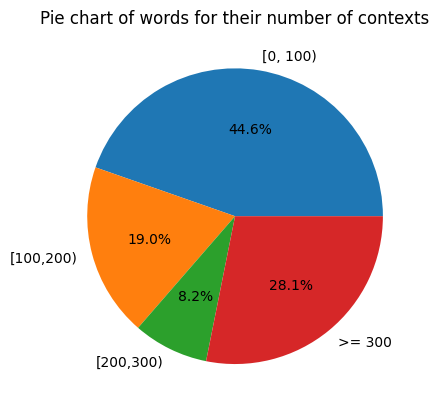
\includegraphics[width=0.7\textwidth]{img/context_pie.png}
    \caption{Number of context words of words in our vocabulary.}
    \label{fig:context_pie}
\end{figure}

When this is the case, removing the underrepresented words from our vocabulary would greatly downsize our training data, but possibly facilitate a better learning for the remaining of the words.

The process of low-context removal starts with counting the number of context tokens surrounding the given word in the text for the given window size. If we find that this number is smaller than the predefined threshold, this type will be eliminated from our train data entirely.

After our testing, we figured there was no real advantage introduced by this process, in contrast, we observed a big performance drop in our final model. Therefore this process is removed from the training pipeline in our base model.

\section{Training and validation split}
\label{sec:val_split}

In the earliest versions of our models, we simply used the entire corpus for the learning, then we evaluated our models on similarity and relatedness tasks. After a while, we decided to partition our corpus into two sets, one for validation and one for learning. 

A validation set is useful for monitoring if our model is still learning meaningful patterns from the data, or is just simply starting to memorize it. After all, we are trying to capture contextual relationships of words, not training a model that perfectly fits our selected training corpus. Removing a portion from our training set for some other purpose will decrease the amount of information to learn from, but we concluded that the advantages of this practice are worth the loss of information.

We decided to use $10\%$ of our corpus for the validation. Given that we are already working with a relatively small corpus, we believe that this portion will not affect our learning greatly, but we still have enough data for a fair validation. We also made sure that the validation set does not include words that are not introduced to our model by the training data. The way we make sure of this can be found in Code \ref{code:val_partition}, starting from line number $6$.

\begin{lstlisting}[language=Python, caption=Training and Validation Set Split, label={code:val_partition}]
# Train - Validation split
split_index = int(len(train_words) * val_partition)
validation_words = train_words[:split_index]
train_words = train_words[split_index:]

# Validation set should not introduce new types
exclude_from_val = set(validation_words) - set(train_words)
validation_words = [w for w in validation_words if w not in exclude_from_val]

\end{lstlisting}

We will show how we perform our validation later in this chapter.

It should be noted that in the majority of machine learning training procedures, it is a useful practice to employ \textit{K-Fold Cross Validation}, in order to leverage the advantages of use of a validation set, by also minimizing the cost of reducing the amount of data to learn from. However, this procedure is also rather time-consuming. Since we are dealing with time and computational power limitations, and we are more interested in observing what our model can possibly promise, we leave this technique as a future improvement.

We should note that we did not partition a test set, since we are not really interested in the loss obtained from another piece of text anyway. Our focus in this study is to learn a set of embeddings, that can perform well on and compete against state-of-the-art models in tasks such as similarity, relatedness, or analogy.

\section{Training loop}

Now we proceed to the learning phase. We use Adam optimizer and our custom model and the loss for the training. In some other variants of our base model, we also tested learning rate decay, however for the base model we set the decay rate to $1.0$, which means it is left unchanged.

Throughout the training, we did our best to keep track of everything and save the models that could be useful for our experiments later. We printed out the training and validation loss in regular intervals, and once the learning was concluded we visualized our logs.

The training loop is a nested \verb|for| loop. The outer loop iterates for the number of epochs. We usually ran six epochs, which seems to be even more than enough in some settings. The inner loop iterates over the training batches, which includes positive and negative training samples that are explained in the previous chapter. In each step, first, we calculate loss, backpropagate it, and in some steps, print out the results. After each epoch, we calculate the loss on our validation set. This gives a better idea about our progress achieved in the last epoch. 

Each time we calculate the training or the validation loss, we compare the performance to the best one we encountered up to that time step. If it is the best one we have seen, we save the model for later use. We also save every model we obtain at the end of each epoch.

\section{Context and noise sampling}

Given a target word $w$, for calculating $\myscore{+}{w, u_1, u_2}$ and $\myscore{-}{w, u_1, u_3}$, we need to sample context words from $C(w)$ and noise words from the negative sampling table. 

Let us have a refresher about the training samples we use. A positive training sample is $(w, u_1, u_2)$, where $u_1$ and $u_2$ are different tokens sampled from $C(w)$. A negative training sample is $(w, u_1, u_3)$, where $u_1$ is again sampled from $C(w)$ and $u_3$ is a noise word sampled from the sampling table.

Our training samples are provided in batches by a generator function which we iterate on in our training loop. It takes as input the training set, batch size, context window size ($L$), the number of negative training samples for each positive training sample, and a dictionary that maps a word index to the list of its context words. The last one is only used when low-context removal is enabled.

\begin{lstlisting}[language=Python, caption=Batch generating function - Part 1]
def get_batches(words, batch_size, win_size, neg_samp, idx_to_contexts):

  n_batches = len(words) // batch_size # Number of batches
  words = words[:n_batches * batch_size] # Keep only the number of words to match the bath_size and n_batches

\end{lstlisting}

Then we iterate over the training set with a step size equal to the batch size. At each step of this loop, we generate the positive and the negative training samples and yield one training batch. It starts with creating an empty list for the target word, two lists for context words, and lists used for sampling each sample. The list of the noise words will be created later. 

This generator yields 4 lists, one containing target words, two containing context words, and one containing noise words. The list containing noise words is two-dimensional, and its second dimension is equal to the number of negative samples to be generated per each positive sample (factor $k$).

\begin{lstlisting}[language=Python, caption=Batch generating function - Part 2]
  for idx in range(0, len(words), batch_size): # for each batch in words
    central_words = []  # list containing target words
    context_words1 = []  # list of words in the context, second order
    context_words2 = []  # list of words in the context, third order

    x, y = [], [] # lists that store the target and context words for each training sample
    z = [] # list of tuples that stores the starting and ending indices of each training sample in the x and y lists
    a = 0 # Counter for the total number of training samples seen so far. Used to keep track of the indices in z.
\end{lstlisting}

A training sample is obtained by using the same index in the lists that are generated by this function. In other words, elements corresponding to the same index in each of these lists are used to generate training samples. For example, using an integer $i$, one positive sample is (\verb|central_words[i]|, \verb|context_words1[i]|, \verb|context_words2[i]|). % \verb|central_words|

Next, we go into an inner loop. This time, we iterate for \verb|batch_size| number of target words and generate positive and negative samples for them.

\begin{lstlisting}[language=Python, caption=Batch generating function - Part 3]
    batch = words[idx:idx + batch_size] # one batch; batch_size number of words (unique), starting from index idx

    for ii in range(len(batch)): # in a batch
      batch_x = batch[ii] # target word for a given training sample
      batch_y = get_context(batch, ii, win_size, idx_to_contexts) # list of context words for that target word

      y.extend(batch_y)
      x.extend([batch_x] * len(batch_y)) # target word added, repeated by the number of context words
      z.extend([[a, len(x)]] * len(batch_y)) # a -> starting idx, len(x) -> end index (for one training sample)

      a = a + len(batch_y)
\end{lstlisting}

Here, picking a word $w_{ii}$ as the target word, we collect its context words. Then we create $|C(w_{ii})| * (|C(w_{ii})| - 1)$ many positive samples, where $|C(w_{ii})|$ is the number of words collected from $w_{ii}$'s context window. The function \verb|get_context|, which is called in line 5, is responsible for returning a list of context words for the specified position in the batch. It employs a dynamic window approach, which is explained in the previous chapter.

\begin{lstlisting}[language=Python, caption=Batch generating function - Part 4]
      central_words.extend([batch_x] * len(batch_y) * (len(batch_y) - 1)) # target word repeated by 2 comb of context words in batch

      for i in range(len(batch_y)): # for each context word in the batch
        context_words1.extend([batch_y[i]] * (len(batch_y) - 1)) # each context word, by number of context words

    for i in range(len(z)):
      values = list(range(z[i][0], z[i][1]))
      values.remove(i) # context_words1[i] and context_words2[i] not the same
      for v in values:
        context_words2.extend([y[v]]) # for each context word, every other context word
\end{lstlisting}

Now the sampling of the context words is concluded. Each context word is paired with every other context word to form positive samples. Next, we create negative samples by sampling noise words from the sampling table, to pair with the words in \verb|context_words1[i]|.

\begin{lstlisting}[language=Python, caption=Batch generating function - Part 5]
    negative_examples = np.random.choice(sample_table, size=(len(central_words), neg_samp))  # list of negative samples for each context word
    for i in range(len(context_words1)):
      for j in range(neg_samp):
        while (context_words1[i] == negative_examples[i][j]): # if a noise word is the same with the context
          negative_examples[i][j] = sample_table[random.randint(0, len(sample_table))] # force it to be different than corresponding context sample
\end{lstlisting}

Finally, we yield the training batch.

\begin{lstlisting}[language=Python, caption=Batch generating function - Part 6]
    yield central_words, context_words1, context_words2, negative_examples
\end{lstlisting}

As the outer loop iterates, we keep generating batches, until all the tokens in the training data are processed. Now we share the entire function once more so that indentation is clear for the reader. 

\begin{lstlisting}[language=Python, caption=Batch generating function]
def get_batches(words, batch_size, win_size, neg_samp, idx_to_contexts):

  n_batches = len(words) // batch_size
  words = words[:n_batches * batch_size] # keep only the number of words to match the bath_size and n_batches

  for idx in range(0, len(words), batch_size): # for each batch in words
    central_words = []  # list containing target words
    context_words1 = []  # list of words in the context, second order
    context_words2 = []  # list of words in the context, third order

    x, y = [], [] # lists that store the target and context words for each training sample
    z = [] # list of tuples that stores the starting and ending indices of each training sample in the x and y lists
    a = 0 # Counter for the total number of training samples seen so far. Used to keep track of the indices in z.

    batch = words[idx:idx + batch_size] # one batch; batch_size number of words (unique), starting from index idx

    for ii in range(len(batch)): # in a batch
      batch_x = batch[ii] # target word for a given training sample
      batch_y = get_context(batch, ii, win_size, idx_to_contexts) # list of context words for that target word

      y.extend(batch_y)
      x.extend([batch_x] * len(batch_y)) # target word added, repeated by the number of context words
      z.extend([[a, len(x)]] * len(batch_y)) # a -> starting idx, len(x) -> end index (for one training sample)

      a = a + len(batch_y)

      central_words.extend([batch_x] * len(batch_y) * (len(batch_y) - 1)) # target word repeated by 2 comb of context words in batch

      for i in range(len(batch_y)): # for each context word in the batch
        context_words1.extend([batch_y[i]] * (len(batch_y) - 1)) # each context word, by number of context words

    for i in range(len(z)):
      values = list(range(z[i][0], z[i][1]))
      values.remove(i) # context_words1[i] and context_words2[i] not the same
      for v in values:
        context_words2.extend([y[v]]) # for each context word, every other context word

    negative_examples = np.random.choice(sample_table, size=(len(central_words), neg_samp))  # list of negative samples for each context word
    for i in range(len(context_words1)):
      for j in range(neg_samp):
        while (context_words1[i] == negative_examples[i][j]): # if a noise word is the same with the context
          negative_examples[i][j] = sample_table[random.randint(0, len(sample_table))] # force it to be different than corresponding context sample

    yield central_words, context_words1, context_words2, negative_examples
\end{lstlisting}

Previously, we tried to explain how we form samples using this function. Now that we have covered our implementation, we can finally give a clearer description of the training samples in terms of the yields of our generator.

For an integer $i$,
\begin{itemize}
    \item \verb|central_words[i]|: A target word. The same word is repeated in\\ \verb|central_words[a:b]|, where $i \in [a, b]$.
    \item \verb|context_words1[i]| and \verb|context_words2[i]|: Two different context words, each in the context of \verb|central_words[i]|.
    \item \verb|negative_examples[i]|: A \underline{list} of noise words to pair with the context word \verb|context_words1[i]|.
\end{itemize}

Using these,
\begin{itemize}
    \item A Positive Training Sample: (\verb|central_words[i]|, \verb|context_words1[i]|, \verb|context_words2[i]|)
    \item A Negative Training Sample: (\verb|central_words[i]|, \verb|context_words1[i]|, \verb|negative_examples[i][j]|)
\end{itemize}

\section{Immediate evaluations}
\label{sec:immediate}

Once the training is completed, we are left with the vectors saved during the training for later use. We use these vectors for visualizations and comparisons against each other. These will be presented in the next chapter. Now, we will briefly describe what kind of quick tests we apply to see if our model performs well, or if the training was efficient. These tests are not nearly as formal or meaningful as the ones we will present later, but they are good enough to give an idea.

\subsection{"Pomegranate" Test}
We set three test words: \textit{car}, \textit{automobile}, and \textit{pomegranate}. Throughout the training process, at regular intervals, we use the most current state of our model to calculate the cosine similarity of these three words to each other. 

We should highlight that we do not compare these results to any standard, and we use only three words. However, this procedure still gives us a good idea of whether the model is behaving as we expect and at what point the training starts to become inefficient. Figure \ref{fig:pomegranate-test} shows the results obtained for our base model. We calculate these similarities at every selected number of batches, rather than every epoch, to have a finer-grained view of the progress.

\begin{figure}[ht]
    \centering
    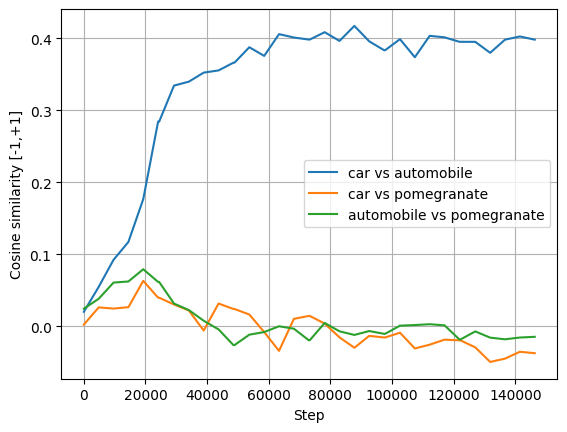
\includegraphics[width=0.6\textwidth]{img/pomegranate-test.png}
    \caption{Pomegranate test during the base model training}
    \label{fig:pomegranate-test}
\end{figure}


\subsection{Closest Neighbors Test}
Another quick test we conduct at the end of the training is checking the closest neighbors for 5 selected words, using the final model. This is an evaluation technique implemented with the inspiration from the article \cite{levy-dependency}, where the authors refer to this technique as "\textit{Qualitative Evaluation}" and use it to show how different models reflect different aspects of words. They limit their observations to 5 neighbors, but we extend it to 10 neighbors. For each word, the closest neighbor appears to be the word itself, we exclude them from the results. These closest neighbors are selected according to the cosine similarity of their target representations to the test word target representation. These five words are \textit{car}, \textit{money}, \textit{flower}, \textit{japan}, and \textit{suspicious}. The results obtained from our base model are given in Table \ref{tab:neighbors_test}.

\begin{table}[ht]
\centering
\begin{tabular}{|c|c|c|c|c|}
\hline
\rowcolor[HTML]{330001} 
{\color[HTML]{FFFFFF} car} & {\color[HTML]{FFFFFF} money} & {\color[HTML]{FFFFFF} flower} & {\color[HTML]{FFFFFF} japan} & {\color[HTML]{FFFFFF} suspicious} \\ \hline
\rowcolor[HTML]{E2EFDA} 
chevrolet                  & demand                       & perennials                    & daigo                        & parchamis                         \\ \hline
cars                       & pricing                      & cultivation                   & taiwan                       & plebs                             \\ \hline
\rowcolor[HTML]{E2EFDA} 
motor                      & dividends                    & sunflower                     & niigata                      & pdpa                              \\ \hline
bmw                        & loans                        & hibiscus                      & korea                        & parcham                           \\ \hline
\rowcolor[HTML]{E2EFDA} 
driver                     & profits                      & petals                        & meiji                        & negotiating                       \\ \hline
nhra                       & tax                          & sepals                        & prefecture                   & confidence                        \\ \hline
\rowcolor[HTML]{E2EFDA} 
motors                     & repay                        & edible                        & japanese                     & khalq                             \\ \hline
automobile                 & bonuses                      & flowers                       & takano                       & blamed                            \\ \hline
\rowcolor[HTML]{E2EFDA} 
chassis                    & cheques                      & shrubs                        & kitakyushu                   & advisers                          \\ \hline
\end{tabular}
\caption{Closest neighbors test on the base model}
\label{tab:neighbors_test}
\end{table}

Note that these neighbors are not listed in a particular order or ranking.